% To familiarize yourself with this template, the body contains
% some examples of its use.  Look them over.  Then you can
% run LaTeX on this file.  After you have LaTeXed this file then
% you can look over the result either by printing it out with
% dvips or using xdvi. "pdflatex template.tex" should also work.
%

\documentclass[oneside]{article}
\setlength{\oddsidemargin}{0.25 in}
\setlength{\evensidemargin}{-0.25 in}
\setlength{\topmargin}{-0.6 in}
\setlength{\textwidth}{6.5 in}
\setlength{\textheight}{8.5 in}
\setlength{\headsep}{0.75 in}
\setlength{\parindent}{0 in}
\setlength{\parskip}{0.1 in}

%
% ADD PACKAGES here:
%

\usepackage{amsmath,amsfonts,graphicx}

%
% The following commands set up the lecnum (lecture number)
% counter and make various numbering schemes work relative
% to the lecture number.
%
\newcounter{lecnum}
\renewcommand{\thepage}{\thelecnum-\arabic{page}}
\renewcommand{\thesection}{\arabic{section}}
\renewcommand{\theequation}{\thelecnum.\arabic{equation}}
\renewcommand{\thefigure}{\thelecnum.\arabic{figure}}
\renewcommand{\thetable}{\thelecnum.\arabic{table}}

%
% The following macro is used to generate the header.
%
\newcommand{\lecture}[4]{
   \pagestyle{myheadings}
   \thispagestyle{plain}
   \newpage
   \setcounter{lecnum}{#1}
   \setcounter{page}{1}
   \noindent
   \begin{center}
   \framebox{
      \vbox{\vspace{2mm}
    \hbox to 6.28in { {\bf 18660 Project Progress Report
	\hfill 22 Apr 2018} }
       \vspace{7mm}
       \hbox to 6.28in { {\Large \hfill Comparison of robust PCA techniques in image and video processing  \hfill} }
       \vspace{4mm}
       \hbox to 6.28in { {\hfill\it Joel Loo, Wang Xueqiang \hfill} }
      \vspace{2mm}}
   }
   \end{center}
   \markboth{Project Progress Report}{Project Progress Report}

   %{\bf Note}: {\it LaTeX template courtesy of UC Berkeley EECS dept.}
   %vspace*{4mm}
}
%
% Convention for citations is authors' initials followed by the year.
% For example, to cite a paper by Leighton and Maggs you would type
% \cite{LM89}, and to cite a paper by Strassen you would type \cite{S69}.
% (To avoid bibliography problems, for now we redefine the \cite command.)
% Also commands that create a suitable format for the reference list.
\renewcommand{\cite}[1]{[#1]}
\def\beginrefs{\begin{list}%
        {[\arabic{equation}]}{\usecounter{equation}
         \setlength{\leftmargin}{2.0truecm}\setlength{\labelsep}{0.4truecm}%
         \setlength{\labelwidth}{1.6truecm}}}
\def\endrefs{\end{list}}
\def\bibentry#1{\item[\hbox{[#1]}]}

%Use this command for a figure; it puts a figure in wherever you want it.
%usage: \fig{NUMBER}{SPACE-IN-INCHES}{CAPTION}
\newcommand{\fig}[3]{
			\vspace{#2}
			\begin{center}
			Figure \thelecnum.#1:~#3
			\end{center}
	}
% Use these for theorems, lemmas, proofs, etc.
\newtheorem{theorem}{Theorem}[lecnum]
\newtheorem{lemma}[theorem]{Lemma}
\newtheorem{proposition}[theorem]{Proposition}
\newtheorem{claim}[theorem]{Claim}
\newtheorem{corollary}[theorem]{Corollary}
\newtheorem{definition}[theorem]{Definition}
\newenvironment{proof}{{\bf Proof:}}{\hfill\rule{2mm}{2mm}}

% **** IF YOU WANT TO DEFINE ADDITIONAL MACROS FOR YOURSELF, PUT THEM HERE:

\newcommand\E{\mathbb{E}}
\newcommand{\compconj}[1]{%
  \overline{#1}%
}

\begin{document}
%FILL IN THE RIGHT INFO.
%\lecture{**LECTURE-NUMBER**}{**DATE**}{**LECTURER**}{**SCRIBE**}
\lecture{1}{0}{1}{Joel Loo, Wang Xueqiang}
\section{Introduction}
Principal components analysis (PCA) and other dimensionality reduction techniques have gained wide traction in the scientific community because of their utility in extracting salient data from large and complex datasets. However an implicit assumption of PCA is that the noise in the data is small and variance from the mean is bounded. Hence, PCA works well on data that is corrupted by small amounts of noise (e.g. data corrupted by Gaussian noise), but can perform poorly on grossly corrupted data and data containing significant outliers.\newline\newline
While there have been many attempts to robustify PCA, many of these methods are heuristics without any optimality guarantees. However, recent advances in low-rank matrix recovery and completion by Candes et al [1], have led to the formulation of robust PCA (RPCA). In RPCA, the problem is reformulated as the recovery of the matrices $L, S$ such that $M = L + S$, where $M$ is the original matrix, $L$ is a low-rank matrix and $S$ is a sparse matrix. Candes et al made the surprising observation that it is possible to perform this decomposition through a tractable convex optimization, if we assume that the low-rank matrix is not simultaneously sparse [1]. In particular, this can be achieved using the Principal Component Pursuit (PCP) estimate which solves the problem
\begin{center}
$
\begin{aligned}
& \underset{L,S}{\text{argmin}}
& & \lVert L\rVert_{*}+ \lambda\lVert S\rVert_{1} 
& \text{subject to}
& & L+S=M
\end{aligned}
$
\end{center}
Since the sparse matrix can have elements of arbitrarily large magnitude, robust PCA thus improves over the PCA technique by allowing the extraction of low-dimensional structure from grossly corrupted data with unbounded outliers. This technique has many important applications in general, and in particular is of great utility in computer vision, where it is used in tackling problems such as background recovery/subtraction (which can be used in video surveillance software), removal of non-Lambertian distortions/specularities/shadows from images (akin to performing inpainting) and even recovery of 3D geometry from low-rank textures in 2D images.\newline\newline
In order to make RPCA practicable on real-world vision systems, a number of reformulations of the problem and improvements have been proposed. Some of these improvements (e.g. Fast PCP [3]) provide significant speed improvements over the method proposed by Candes et al, while others reformulate RPCA as an online algorithm (e.g. online RPCA via stochastic optimization [2], iFrALM).
\section{Problem Statement}
In this project, we aim to survey several RPCA algorithms - in particular we will implement these algorithms and compare their performance, in terms of both speed and ability to separate low-rank structure from sparse noise. We are primarily interested in applying these algorithms to, and testing them on vision applications. Two applications that we are particularly interested in are the removal of specularities/non-Lambertian distortions from images, as well as background recovery/subtraction in videos. Background recovery/subtraction in video streams provides an interesting case study for RPCA as well, since it is desirable to have both algorithms that can separate backgrounds in post-processing as well as on the fly. To this end, we will use this particular application to benchmark the performance of both RPCA algorithms that offer significant speed-ups, as well as RPCA algorithms formulated to be online in nature. We will perform the implementations and benchmarking described above in Python, with code available on the private Github repository https://github.com/joelloo/18660\_project
\section{Algorithm implementation and comparison}
\subsection{Standard RPCA algorithms}
The formulation of RPCA by Candes et al aims to solve the convex problem
\begin{center}
$
\begin{aligned}
& \underset{L,S}{\text{argmin}}
& & \lVert L\rVert_{*}+ \lambda\lVert S\rVert_{1} 
& \text{subject to}
& & L+S=M
\end{aligned}
$
\end{center}
There have been several approaches taken to solving this original formulation as summarized in [4]. These include a principal component pursuit that is effectively an exact Augmented Lagrangian Multiplier (ALM) method, an inexact ALM method, and an accelerated proximal gradient approach [5].
\subsection{Fast PCP}
The Fast PCP method [3] reformulates the original convex PCP problem. The original formulation (solved with standard RPCA methods) tends to be rather computationally expensive as we have observed. The Fast PCP method on the other hand changes the PCP constraint $M = L+S$ to the Frobenius-norm penalty $\lVert L+S-M\rVert_{F}$, and changes the nuclear norm penalty to a constraint, i.e. $\lVert L\rVert_{*} \le t$, for some $t$ that is small compared to the dimensions of $M$. The nuclear norm constraint is reformulated as a constraint on the rank, yielding
\begin{center}
$
\begin{aligned}
& \underset{L,S}{\text{argmin}}
& & \lVert L+S-M\rVert_{F}+ \lambda\lVert S\rVert_{1} 
& \text{subject to}
& & \text{rank}(L) = t
\end{aligned}
$
\end{center}
This optimization problem over two variables is easily amenable to an alternating minimization procedure $
L_{k+1}  =\begin{aligned}
& \underset{L,S}{\text{argmin}}
& & \lVert L_{k}+S_{k}-M\rVert_{F}
& \text{subject to}
& & \text{rank}(L_{k}) = t
\end{aligned}
$ and $S_{k+1} = \begin{aligned}
& \underset{L,S}{\text{argmin}}
& & \lVert L_{k+1}+S_{k}-M\rVert_{F}+ \lambda\lVert S\rVert_{1} 
\end{aligned}
$. The first minimization is recognizable as a rank-constrained least squares problem, for which the canonical solution is to compute the partial SVD, i.e. $L_{k+1} = u*s*vt$, where $u$ is the first $t$ columns of $U$, $s$ is the first square submatrix of $\Sigma$ of dimension $t$, $vt$ is the first $t$ rows of $V^{T}$ and  $M-S_{k} = U\Sigma V^{T}$. We used scikit-learn's randomized\_svd function to compute the partial SVD in our implementation. The second minimization can be solved by direct application of the soft thresholding operator. The algorithm consists primarily of these two steps, where the main bottleneck is the SVD. Since we are only computing a partial SVD for only a small number of columns/rows (if we enforce low rank on $L$) this method is very fast in practice. To enforce low rank in $L$, we also implement a check, wherein we compute the contribution of each successive singular value, and stop increasing the rank when the singular value becomes too small.\newline\newline
\subsection{Online RPCA via stochastic optimization (STOC-RPCA)}
\subsection{Incremental Fixed-rank RPCA}
As stated before, robust PCA solver can lead to exoensive computation without an efficient algorithm. Robust PCA's application to Video background recovery can also be impractical when the frames accumulate to the place where a computer's memory is hard to reach. To reduce the computation expense and to make online backgroung recovery pratical. Jian [6] presented an algorithm called iFrALM (incremental fixed-rank ALM). The algorithm splits the frames into an initial batch and an incremental batch. The algorithm will only save fixed-rank components of initial batch and some more memory to save the incremental batch. Whena a new video frame batch arrives, the algorithm updates the principle component in an incremental way and therefore saves computation cost and memory cost.

Before introducing the iFrALM algorithm, we would like to introduce the iSVD(incremental SVD) method [7] first. This is what iFrALM is based on, as most robust PCA algorithms are based on SVD. Incremental SVD is a method to update the matrix's SVD with new-added part based on the original matrix's SVD, specially in video backgroud recovery, to update the matrix's SVD with new-added columns. Incremental FrALM implements the iSVD method presented by Zha. The problem si formulated as:
\begin{align*}
\text{Given A $ \in R^{m \times n}$ is the original term document matrix and } A_k &= P_k \Sigma_k Q_k^T \\ \text{Let D $\in R^{m \times p}$ Compute the best rank-k approximation of} B &\equiv [A_k, D]
\end{align*}
More details can be found in Zha's paper.
In FrALM, the robust problem is formulated as:
\[\min\limits_{A,E}{\|E\|_F}, \text{subject to rank(A) = known r, D = A + E}\]
$\|\dot\|_F$ is the Frobenius norm, D is the original matrix, A and E are priciple data matrix and sparse data matrix. FrALM uses SVD to minimize the equation with A being factorized as $A = U^r S^r {V^r}^T$.

In iFrRPCA, D is seperated into initial batch $D_0$  and incremental batches $D_1, D_2, D_i, \cdots$. Then following the FrALM, we can solve each batch size and get the principle component of A: $A_{i- 1} = U_{i-1} S_{i-1} V^T_{i-1}$, pass the $A_{i-1}$ into next problem, that is to minimize E with $D = [A_{i -1}, D_i]$. In the new problem, iSVD will help us to get the new SVD update with both efficient computation and memory.

However, during the implementation, because the author did not give an explict convergence condition along with the parameters used in the algorithm, although we have built the programming structure, it takes time to test out proper parameters. Another problem during the implementation is that video frames usually have a large size. We spend some time and still need to spend more in solving this problem in folling steps. Even we meet some problems, these problems will just be a matter of time, knowing the reason behind these, we will solve these problems.



\subsection{Comparison}
So far, we are trying to test our algorithms on high resolution image, we make a simpel test on low resolution image which is a highway.The results are as below:

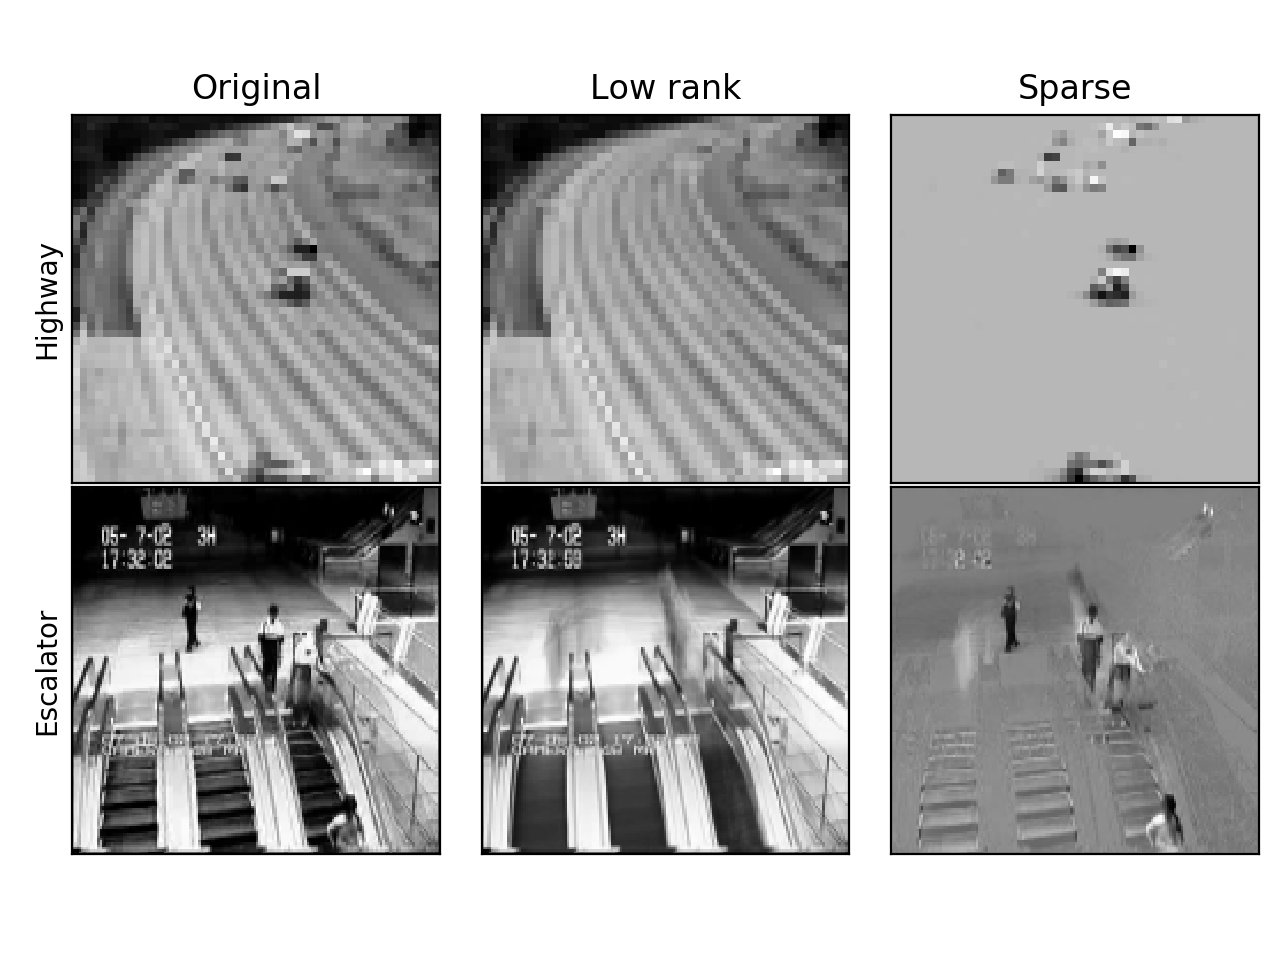
\includegraphics[scale = 0.5]{montage_fpcp.png}

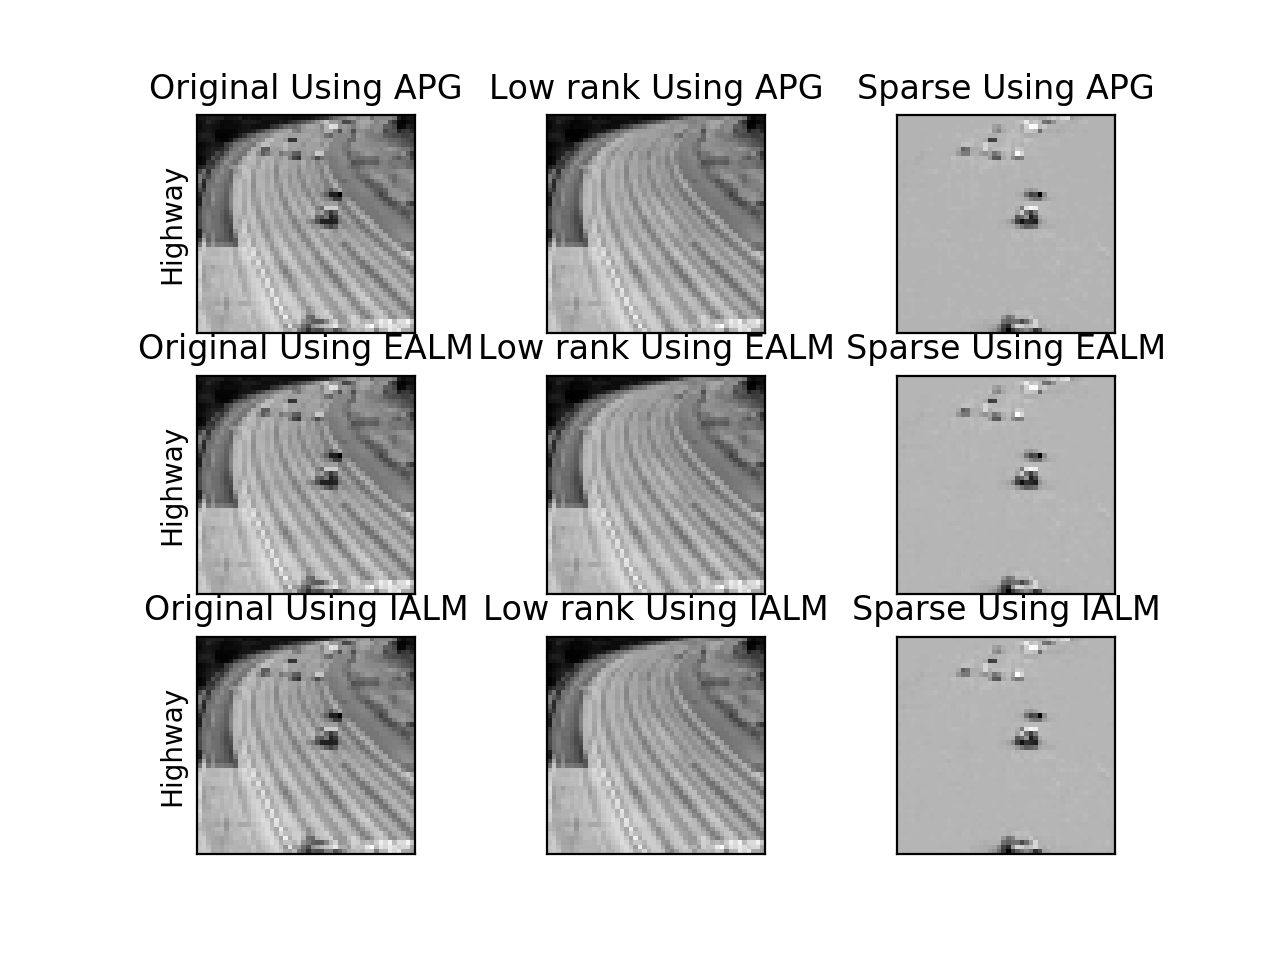
\includegraphics[scale=0.5]{compare.png}

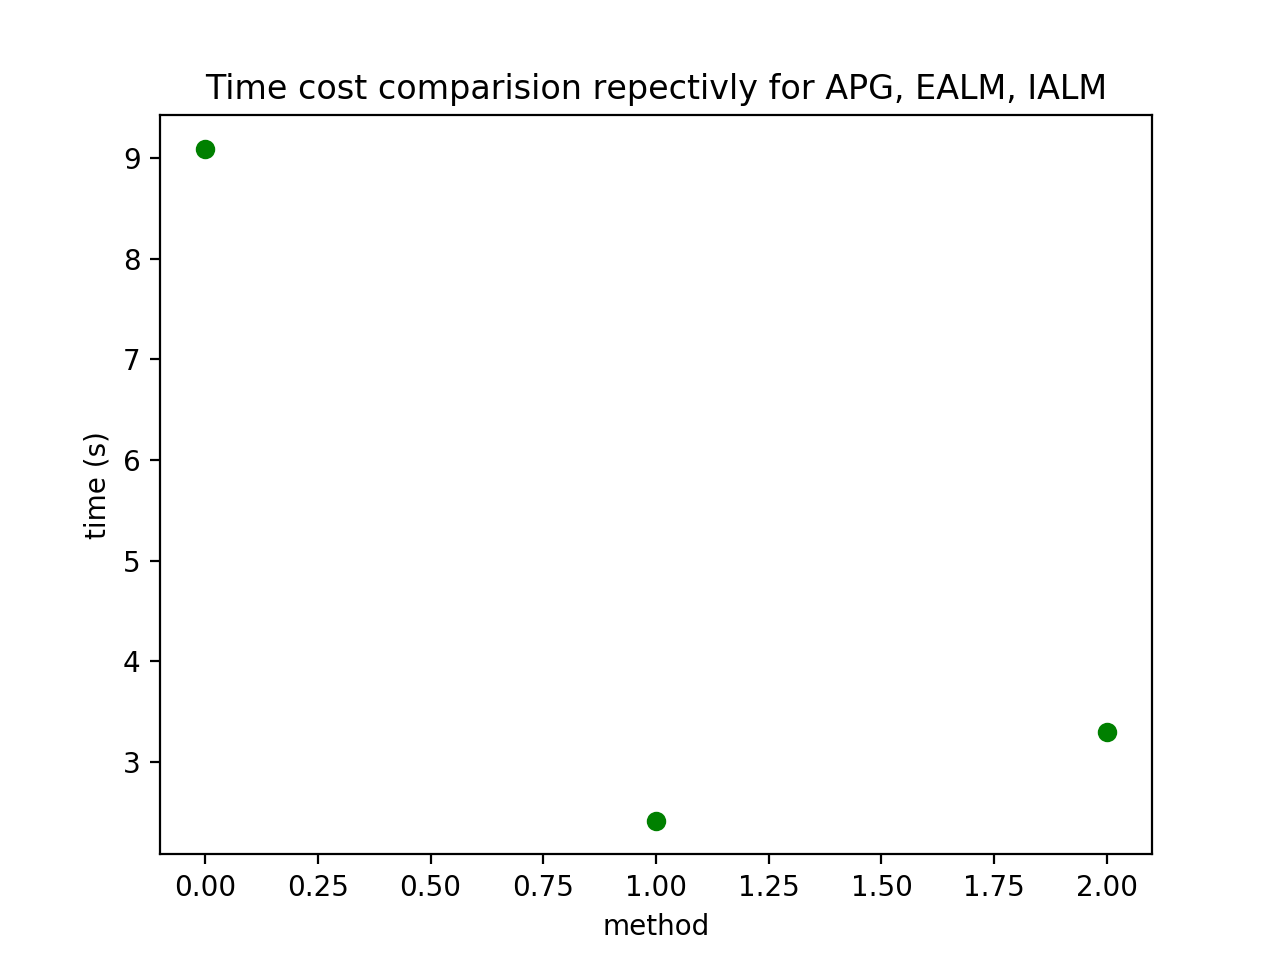
\includegraphics[scale=0.5]{timecost.png}




\section{Next steps}
We have two primary goals going forward. Firstly, we want to perform more detailed benchmarking, analysis and comparison of the algorithms we have presently implemented. In particular, we want to test our algorithms on a wider variety of video streams (e.g. videos with larger images, longer videos etc.) to observe how the algorithms scale and how close the algorithms can get to real-time performance. Additionally, we could improve on the way in which we currently benchmark the quality of the low-rank and sparse separation. This is currently done by visual inspection of the results of our implementations when applied to specularity removal or background subtraction. While we are able to get a general sense of how performant our algorithm is from this, we would like to take a more quantifiable approach. We could do this by generating low-rank data and corrupting it with arbitrary sparse data and quantifying the separation by seeing if the algorithm is able to return a rank close to that of our artificial low-rank data, and also by computing the distance of the computed low-rank and sparse matrices from our artificially created low-rank and sparse matrices using the Frobenius norm or some other metric.\newline\newline
Secondly, we would like to explore how close we can get to real-time performance when implementing background recovery/subtraction with RPCA. While Fast PCP is fast and highly performant, it is not adapted for real-time continuous background recovery/subtraction such as in video surveillance. This is because it ultimately uses all the frames in the video to perform the low-rank extraction, which might be slow and unwieldy for the large numbers of frames present in a surveillance video. For this purpose, we might desire an online algorithm that incorporates frames as they come in, such as we have with STOC-RPCA (but which is slower than Fast PCP, because it performs more computations). One idea we have to do this would be to adapt Fast PCP such that it operates on a fixed number of frames, i.e. Fast PCP would be continuously applied to a moving window of frames as more frames comes in, giving it a continuous real-time ability, and possibly giving it the ability to adapt better to permanent changes to the background. Rodriguez and Wohlberg have proposed extensions to Fast PCP to enable incremental updating, in a similar spirit to what we propose. If we have the time, we would like to attempt implementing their paper and comparing the performance of their algorithm to our suggestion and the other algorithms we have implemented.
\newline\newline
However, we also would like to explore the possibility of combining some aspects of Fast PCP and STOC-RPCA. Both Fast PCP and STOC-RPCA reformulate the original PCP optimization problem. The main difference between the formulations is that the nuclear norm penalty in STOC-RPCA is a rank constraint in Fast PCP. We are curious to see if we are able to reconcile these differences in the formulation and hence the algorithms, and try to reformulate the Fast PCP algorithm such that the low-rank and sparse matrix can be updated frame by frame.

\section{References}
[1] \hspace*{8pt} E. Candes, X. Li, Y. Ma, and J. Wright, "Robust principal component analysis?," Journal of the ACM, vol. 58,
no. 3, May 2011.

[2] \hspace*{8pt}Online Robust PCA via Stochastic Optimization	(Feng, Xu and Yan, 2013). Reference: Feng, Jiashi, Huan Xu, and Shuicheng Yan. "Online robust pca via stochastic optimization." Advances in Neural Information Processing Systems. 2013.

[3] \hspace*{8pt}P. Rodriguez and B. Wohlberg, "Fast principal component pursuit via alternating minimization," in IEEE ICIP, Melbourne, Australia, Sep. 2013, pp. 69–73.

[4] \hspace*{8pt}Guyon, C., Bouwmans, T., and Zahzah, E. (2012). Robust Principal Component Analysis for Background Subtraction: Systematic Evaluation and Comparative Analysis.

[5] \hspace*{8pt}Lin, Z., Ganesh, A., Wright, J., Wu, L., Chen, M., and Ma, Y. (2009). Fast convex optimization algorithms for exact recovery of a corrupted low-rank matrix. Intl. Workshop on Comp. Adv. in Multi-Sensor Adapt. Processing, Aruba, Dutch Antilles.

[6] \hspace*{8pt}Jian Lai, Wee Kheng Leow, Terence Sim (2015). Incremental Fixed-Rank Robust PCA for Video Backgroud Recovery

[7] \hspace*{8pt}Hongyuan Zha, Horst D. Simon (1999). On Updating Problems in Latent Semantic Indexing


\end{document}





